\scanpage{341}

Of course, this character will again be called, ``multiplier'', \unsure{and|or} ``cyclotomic character''. \deleted{\unsure{It}} If our fundamental conjecture is true, this character identifies $(\Gamma_\Sigma)_{\mathrm{ab}}$ with $\widehat{\mathbb Z}^{*}$.

On the other hand, if $I=I(\pi)$, the canonical homomorphism
\[
\widehat{\widehat{\mathcal T}}\longrightarrow\unsure{\mathfrak S_I|\mathcal S_I}
\]
is \deleted{\illegible{1}} not trivial on $\Sigma$, but induces a surjective homomorphism
\[
\Sigma\longrightarrow\mathfrak S_I^{\deleted{\unsure{!}}}
\]
whence a subgroup $\Sigma^!$ such that
\[
\Sigma/\Sigma^!\xrightarrow{\sim}\mathfrak S_I.
\]
\margin{\unsure{morally}, $\Sigma^!\simeq\widehat{\mathcal T}^{!+}$}

We see at once that $\forall\ \unsure{\gamma|g}\in\widehat{\widehat{\mathcal T}}$ which normalizes $\Sigma$ normalizes $\Sigma^!=\Sigma\cap\widehat{\widehat{\mathcal T}}^!$, \unsure{whence|i.e.} $\Sigma^!$ is also invariant in $\mathcal N_\Sigma$. \deleted{\illegible{3}} Let $\mathcal N_\Sigma^!=\mathcal N_\Sigma\cap\widehat{\widehat{\mathcal T}}^!$, we have a Cartesian diagram of subgroups of $\widehat{\widehat{\mathcal T}}$
\diagram{\begin{tikzcd}[ampersand replacement=\&]
\mathcal N^!\arrow[r,hook,"\mathfrak S_I"] \& \mathcal N\\
\Sigma^!\arrow[u,hook,"\Gamma_\Sigma"]\arrow[r,hook,"\mathfrak S_I"'] \& \Sigma\arrow[u,hook,"\Gamma_\Sigma"']
\end{tikzcd}}
giving an injective homomorphism
\[
\mathcal N/\Sigma^!\longrightarrow
\underbrace{\mathcal N/\mathcal N^!}_{\mathfrak S_I}\times
\underbrace{\mathcal N/\Sigma}_{\Gamma_\Sigma}
\]
\unsure{of which|when} we see at once that it is bijective
\margin{\unsure{and|for} $\unsure{\Sigma}/\Sigma^!\xrightarrow{\sim}\mathcal N/\mathcal N^!\ (\simeq\mathfrak S_I)$}
\[
\mathcal N/\Sigma^!\xrightarrow{\sim}\mathcal N/\mathcal N^!\times\mathcal N/\Sigma\simeq\mathfrak S_I\times\Gamma_\Sigma
\]
and consequently we also have
\[
\unsure{\mathcal N}^!/\Sigma^!\xrightarrow{\sim}\mathcal N/\unsure{\Sigma}=\Gamma_\Sigma,
\]
i.e. the group $\Gamma_\Sigma$ of \unsure{arithmetically} outer automorphisms of $(\pi,\Sigma)$ can also be described via the automorphisms
\mspage{340}

\scanpage{342}
\mspage{173}

that are outer and induce the identity on $I$.

In the case $(g,\nu)=(0,3)$, we have $\Sigma^!=(1)$, \unsure{$\Rightarrow$} hence $\Sigma\xrightarrow{\sim}\mathfrak S_3$. $\mathcal N$ is the \deleted{product} normalizer of $\mathfrak S_3$ in $\widehat{\widehat{\mathcal T}}$, $\mathcal N^!$ \inserted{$\unsure{\xrightarrow{\sim}}\Gamma_\Sigma$} is its centralizer, and $\mathcal N$ is identified with the direct product of the two.

\deleted{\illegible{2}}

Now let $\unsure{I|I'}\subset I$, \inserted{$\nu'=\operatorname{card}I'$,} and let us consider the outer group $\pi'$ obtained from $\pi$ by ``plugging the holes at $\unsure{I\setminus I'}$'', whence a homomorphism
\[
\pi^{\unsure{*}}\longrightarrow\pi'.
\]
\deleted{\unsure{For a map}} \inserted{Let us consider} the bases \inserted{of $\pi$,} for which \deleted{$l_{\nu-\nu'+1}\ldots l_\nu$} \deleted{\illegible{2}} \inserted{the $\nu'$ \deleted{last} \inserted{first} $l_i$,} are in \inserted{\deleted{\unsure{bases}}} groups \unsure{with} loops \deleted{\unsure{in}} $L_{i'}$ $(i'\in I')$ --- we call them adapted to $I'$; they form a torsor \inserted{$\subset\operatorname{Isom}_{\mathrm{lac}}(\widehat\pi_{g,\nu},\pi)$} under the subgroup of \deleted{\illegible{1}} $\unsure{\widehat{\widehat{\mathcal G}}}_{g;(\nu,\nu'\deleted{\unsure{+2}})}$ of $\widehat{\widehat{\mathcal G}}_{g,\nu}$ \inserted{$=\operatorname{Aut}\deleted{\,\mathrm{ext}}_{\unsure{\mathrm{lac}}}(\widehat\pi_{g,\nu})$} \inserted{consisting} of the $\unsure{u|h}\in\widehat{\widehat{\mathcal G}}_{g,\nu}$ whose image in $\mathfrak S_I$ \unsure{leaves invariant} \inserted{\deleted{\unsure{also}} the set} of the $\nu'\deleted{\unsure{+2}}$ first elements (\unsure{or}, of the $\nu-\unsure{\nu'}$ last \inserted{\unsure{its|their} complementary set,}).

\margin{Whence also: $\forall$ basis, $\forall$ discretification, oriented discretification of $\pi$ defines one of $\pi'$, whence \unsure{ditto} for classes of \inserted{$\pi,\pi'$} conjugation, i.e. \unsure{for|by} the strict prediscretifications \inserted{(possibly oriented)}, and also \unsure{for|by} the closures of the classes, i.e. the \deleted{\illegible{1}} prediscretifications and oriented prediscretifications. It is only the case of \unsure{arithmetizations|arithmetizations} that \deleted{\unsure{requires}} \inserted{\unsure{would require}} a finer analysis\ldots}

For such a basis, we find a corresponding basis of $\pi'$. \deleted{the passage} The datum of $(\pi,I')$ is equivalent to that of a torsor under $\widehat{\widehat{\mathcal G}}_{g,(\nu,\nu'\deleted{\unsure{+2}})}$, that of a $\pi'$ to \deleted{\illegible{1}} the datum of a torsor under $\widehat{\widehat{\mathcal G}}_{g,\nu'}$, and the passage from $\pi$ to $\pi'$ is described by the change of group of operators
\[
\widehat{\widehat{\mathcal G}}_{g,(\nu,\nu')}\longrightarrow\widehat{\widehat{\mathcal G}}_{g,\nu'}
\]
this homomorphism sends $\underset{\inserted{\substack{\cap\\ \Sigma_{g,\nu}}}}{\widehat{\mathcal G}_{g,(\nu,\nu')}}\inserted{=\Sigma_{g,(\nu,\nu')}}$ into $\unsure{\widehat{\mathcal G}}_{g,\nu'}=\Sigma_{g,\nu'}$,
\mspage{341}

\scanpage{343}

\inserted{and even} $\mathcal G_{g,(\nu,\nu')}$ into $\mathcal G_{g,\nu'}$, also $\pi$ into $\pi'$. It follows that every prediscretification of $\pi$ defines one of $\pi'$, the same for strict prediscretifications, \deleted{bases} discretifications, outer bases \inserted{``adapted to $I'$'' \deleted{\unsure{(i.e.) for which}}}. Finally, if we have a ``prearithmetization'' of $\pi$, i.e. a $\Sigma\subset\widehat{\widehat{\mathcal T}}(\pi)$, do we deduce from it a prearithmetization of $\pi'$ --- i.e. \inserted{\unsure{(for example)}} if two prediscretifications of $\pi$ are compatible i.e. \deleted{\unsure{define}} have the same group $\Sigma\subset\widehat{\widehat{\mathcal T}}(\pi)\unsure{,}$ of outer automorphisms, is the same true of their images?

\deleted{\unsure{[}The question comes down to this:\unsure{]}
\unsure{[}the homomorphism
\[
\widehat{\widehat{\mathcal T}}_{g,(\nu,\nu')}
\longrightarrow\widehat{\widehat{\mathcal T}}_{g,\nu'},
\]
\unsure{which sends}
\[
\widehat{\mathcal T}_{g,(\nu,\nu')}=\unsure{\Sigma}_{g,(\nu,\nu')}
\]
into]}

To see more clearly, we are going to write in diagram form the remarkable sets associated with $\pi$, and this in two ways, one without using any \unsure{particular structure|particular structures} on $I=I(\pi)$, the other using a total order, which makes it possible, in the torsor $\operatorname{Isom}_{\mathrm{lac}}(\widehat\pi_{g,\nu},\pi)$ under $\widehat{\widehat{\mathcal G}}_{g,\nu}$, to define the subtorsor under $\widehat{\widehat{\mathcal G}}_{g,\nu}^{!}$ which we may denote \deleted{\illegible{1}} $\operatorname{Isom}_{\mathrm{lac}}^{!}(\widehat\pi_{g,\nu},\pi)$.
\mspage{342}

\scanpage{344}
\mspage{174}

\diagram{
\begin{tikzcd}[ampersand replacement=\&,column sep=large,row sep=large]
\& \&
\begin{gathered}
\text{Bases of }(\pi)\simeq\operatorname{Isom}_{\mathrm{lac}}(\widehat{\pi}_{g,\nu},\pi)\\
\downarrow\\
[\text{Bases}^{!}(\pi)\simeq\operatorname{Isom}^{!}_{\mathrm{lac}}(\widehat{\pi}_{g,\nu},\pi)]
\end{gathered}
\arrow[dl,"\mathcal G^{+}_{g,\nu}"']\arrow[dr,"\widehat{\pi}_{g,\nu}"]
\&\\
\&
\begin{gathered}
\text{discretifications}\ \inserted{\text{oriented}}\ (\pi)\\
\simeq\operatorname{Isom}_{\mathrm{lac}}(\widehat{\pi}_{g,\nu},\pi)/\mathcal G^{+}_{g,\nu}\\
\simeq\operatorname{Isom}^{!}_{\mathrm{lac}}(\widehat{\pi}_{g,\nu},\pi)/\mathcal G^{!+}_{g,\nu}
\end{gathered}
\arrow[dl,"\{\pm1\}"']\arrow[dr]
\&\&
\begin{gathered}
\text{Outer bases of }\pi\\
\simeq\operatorname{Isom}\deleted{\,\mathrm{ext}}_{\mathrm{lac}}(\widehat{\pi}_{g,\nu},\pi)/\widehat{\pi}_{g,\nu}\\
\simeq\operatorname{Isom\,ext}_{\mathrm{lac}}(\widehat{\pi}_{g,\nu},\pi)\\
\downarrow\\
[\text{Outer bases}^{!}(\pi)\simeq\operatorname{Isom\,ext}^{!}_{\mathrm{lac}}(\widehat{\pi}_{g,\nu},\pi)]
\end{gathered}
\arrow[dl,"\mathcal T_{g,\nu}"]\\
\left[\begin{gathered}\text{Discretifications }(\pi)\\\simeq\end{gathered}\right]
\arrow[d]
\&\&
\begin{gathered}
\text{prediscretifications}\ \inserted{\text{oriented}}\ \text{strict}\ (\pi)\\
\simeq\operatorname{Isom}_{\mathrm{lac}}(\unsure{\widehat{\pi}}_{g,\nu},\pi)/\mathcal G^{+}_{g,\nu}\cdot\widehat{\pi}_{g,\nu}\\
\simeq\operatorname{Isom\,ext}_{\mathrm{lac}}(\widehat{\pi}_{g,\nu},\pi)/\mathcal T^{+}_{g,\nu})\\
\simeq\operatorname{Isom}^{!}(\widehat{\pi}_{g,\nu},\pi)/\mathcal G^{!+}_{g,\nu}\cdot\widehat{\pi}_{g,\nu}\\
\simeq\operatorname{Isom\,ext}_{\mathrm{lac}}(\widehat{\pi}_{g,\nu},\pi)/\mathcal T^{!+}_{g,\nu}
\end{gathered}
\arrow[dll,"\{\pm1\}"']\arrow[d]
\&\\
\left[\begin{gathered}\text{strict prediscretifications}\\\text{of }\pi\\\simeq\end{gathered}\right]
\&\&
\begin{gathered}
\text{prediscretifications}\ \inserted{\text{oriented}}\ (\pi)\\
\simeq\operatorname{Isom}_{\mathrm{lac}}(\widehat{\pi}_{g,\nu},\pi)/\widehat{\mathcal G}^{+}_{g,\nu}\\
\simeq\operatorname{Isom\,ext}_{\mathrm{lac}}(\widehat{\pi}_{g,\nu},\pi)/\widehat{\mathcal T}^{+}_{g,\nu}\\
\deleted{\unsure{\simeq}}\quad
\simeq\operatorname{Isom}^{!}_{\mathrm{lac}}(\widehat{\pi}_{g,\nu},\pi)/\widehat{\mathcal G}^{!+}_{g,\nu}\\
\simeq\operatorname{Isom\,ext}^{!}_{\mathrm{lac}}(\widehat{\pi}_{g,\nu},\pi)/\widehat{\mathcal T}^{!+}_{g,\nu}
\end{gathered}
\arrow[dll,"\{\pm1\}"']\arrow[dd,"\Gamma_{\Sigma}"',"\Gamma_{g,\nu}"]
\&\\
\left[\begin{gathered}\text{prediscretifications of }\pi\\\simeq\end{gathered}\right]
\arrow[drr]
\&\&\&\\
\&\&
\begin{gathered}
\text{prearithmetizations of }\pi\\
\simeq\operatorname{Isom}_{\mathrm{lac}}(\widehat{\pi}_{g,\nu},\pi)/\mathcal M_{g,\nu}\\
\simeq\operatorname{Isom\,ext}_{\mathrm{lac}}(\widehat{\pi}_{g,\nu},\pi)/\mathcal N_{g,\nu}\\
\simeq\operatorname{Isom}^{!}_{\mathrm{lac}}(\widehat{\pi}_{g,\nu},\pi)/\mathcal M^{!}_{g,\nu}\\
\simeq\operatorname{Isom\,ext}^{!}_{\mathrm{lac}}(\widehat{\pi}_{g,\nu},\pi)/\mathcal N^{!}_{g,\nu}
\end{gathered}
\&
\end{tikzcd}
}

\margin{\unsure{not separated}}
\margin{\unsure{not separated}}
\margin{\diagram{\begin{tikzcd}[ampersand replacement=\&]
\deleted{\left\downarrow\vphantom{\rule{0pt}{2.8cm}}\right.}
\end{tikzcd}}}
\margin{\diagram{\begin{tikzcd}[ampersand replacement=\&,column sep=0.35cm,row sep=1.4cm,cells={nodes={inner sep=0pt,minimum size=0pt}}]
{} \& {} \arrow[d,bend right=8,line width=0.8pt,
  "{\widehat{\mathcal T}_{g,\nu}}"{pos=0.95,right}] \\
{} \& {} \arrow[dl,bend right=8,no head,line width=0.3pt] \\
{} \& {}
\end{tikzcd}}}
\margin{\diagram{\begin{tikzcd}[ampersand replacement=\&,column sep=0.30cm,row sep=0.40cm,cells={nodes={inner sep=0pt,minimum size=0pt}},arrows={line width=0.65pt,start anchor=center,end anchor=center,shorten <=1.2pt,shorten >=1.2pt}]
{} \& {} \& {} \arrow[dl] \arrow[dr] \& {} \& {} \arrow[ll] \arrow[dr] \& {} \\
|[yshift=-0.05cm]| {} \arrow[dr] \& {} \arrow[l] \arrow[dr] \& {} \& {} \arrow[dl] \& {} \& {} \arrow[ll] \\
{} \& |[yshift=-0.04cm]| {} \arrow[d] \& {} \arrow[l] \arrow[d] \& {} \& {} \& {} \\
{} \& |[yshift=-0.06cm]| {} \arrow[dr] \& {} \arrow[l] \arrow[dd,line width=1.25pt] \& {} \& {} \& {} \\
{} \& {} \& |[xshift=-0.12cm,yshift=-0.25cm]| {} \& {} \& {} \& {} \\
{} \& {} \& |[yshift=-0.45cm]| {} \& {} \& {} \& {}
\end{tikzcd}}}
\margin{Please turn over}
\mspage{343}

\scanpage{345}

\uline{N.B.}

We set \deleted{\illegible{1}}
\[
\Gamma_{g,\nu}=\mathcal N_{g,\nu}/\Sigma_{g,\nu}
=\mathcal N^{!}_{g,\nu}/\Sigma^{!}_{g,\nu}
\]
(where $\Sigma_{g,\nu}=\widehat{\mathcal T}^{+}_{g,\nu}$,
$\Sigma^{!}_{g,\nu}=\widehat{\mathcal T}^{!+}_{g,\nu}$).
We can also describe it as the group $\Gamma_{\Sigma}$ associated with a
profinite \inserted{outer} group with loops \inserted{$\pi$}
\uline{equipped} with an \inserted{oriented} prediscretification
$\alpha$ (nothing more). If we have two such \deleted{groups}\inserted{pairs}
$(\pi,\alpha),(\pi',\alpha')$, \unsure{whence} $\Gamma_{\Sigma}$ and
$\Gamma_{\Sigma'}$ ($\Sigma=\operatorname{Aut\,ext}_{\mathrm{lac}}(\pi,\alpha)$,
$\Sigma'=\operatorname{Aut\,ext}_{\mathrm{lac}}(\pi',\alpha')$), we indeed find a
\uline{canonical} isomorphism
\[
\Gamma_{\Sigma}\xrightarrow{\sim}\Gamma_{\Sigma'}
\]
by taking any outer isomorphism \inserted{with loops $u$} of $\pi$ with $\pi'$,
transforming $\alpha$ into $\alpha'$ --- the associated isomorphism
$\Gamma_{\Sigma}\longrightarrow\Gamma_{\Sigma'}$ obviously does not depend on the choice of
$u$.

This being said, the \inserted{pairs $(\pi,\Sigma)$ of a}
\unsure{profinite|profinite} \unsure{group|groups} with loops of type $(g,\nu)$,
\deleted{equipped with a}\inserted{\unsure{equipped with a}} prearithmetization,
with as morphisms the \unsure{arithmetically} outer \unsure{isomorphisms}
\deleted{transforming}\inserted{(relative to} $\Sigma$ and $\Sigma'\ldots$),
form a connected groupoid $\Pi_{g,\nu}$, having an ``origin'' object
(defined up to unique isomorphism as being $(\widehat{\pi}_{g,\nu},\Sigma_{g,\nu})$,
\unsure{or at will} any $(\pi,\Sigma_{\alpha})$ coming from a
$(\pi,\alpha)$ ($\alpha$ an oriented prediscretification of $\pi$),
and whose group \unsure{of} \unsure{automorphisms} is precisely $\Gamma_{g,\nu}$.
\mspage{344}

\scanpage{346}
\mspage{175}

We observe that, with the exception of the two homogeneous spaces
(under $\widehat{\widehat{\mathcal G}}(\pi)$, but not \unsure{necessarily|necessarily} under
$\widehat{\widehat{\mathcal G}}(\pi,I')$, or even under
$\widehat{\widehat{\mathcal G}}^{!}(\pi)$) Bases $(\pi)$ and Outer bases $(\pi)$,
the other four are in fact homogeneous spaces under
$\widehat{\widehat{\mathcal G}}^{!}$, and are expressed as quotients of the
\inserted{$\widehat{\widehat{\mathcal G}}^{!}_{g,\nu}$-}torsor
$\operatorname{Isom}^{!}(\widehat{\pi}_{g,\nu},\pi)$, by the four subgroups
\[
\mathcal G^{!}_{g,\nu},\quad
\mathcal G^{!}_{g,\nu}\cdot\widehat{\pi}_{g,\nu},\quad
\widehat{\mathcal G}^{!}_{g,\nu},\quad
\mathcal M^{!}_{g,\nu}
\]
(the last defined as the inverse image of $\mathcal N^{!}_{g,\nu}$ in
$\widehat{\widehat{\mathcal G}}_{g,\nu}$, just as $\mathcal M_{g,\nu}$ is defined
as the inverse image of $\mathcal N_{g,\nu}$).
We find on the other hand, \unsure{if|for} $I'=\{i_0,\ldots,i_{\nu'-1}\}$,
\unsure{a|some} homomorphism
\[
\widehat{\widehat{\mathcal G}}^{!}_{g,\nu}\longrightarrow
\widehat{\widehat{\mathcal G}}^{!}_{g,\nu'},
\]
sending $\mathcal G^{!}_{g,\nu}$ into $\mathcal G^{!}_{g,\nu'}$,
\deleted{\illegible{1} $\unsure{\widehat{\mathcal G}}_{g,\nu}$ into
$\unsure{\widehat{\pi}_{g,\nu}}$}
by sending $\pi_{g,\nu}$ into $\pi_{g,\nu'}$, thus $\widehat{\pi}_{g,\nu}$
into $\widehat{\pi}_{g,\nu'}$,
$\widehat{\mathcal G}^{!}_{g,\nu}=\Sigma^{!}_{g,\nu}$ into
$\widehat{\mathcal G}^{!}_{g,\nu'}=\Sigma^{!}_{g,\nu'}$, and the subgroup
$\mathcal G^{!}_{g,\nu}\cdot\widehat{\pi}_{g,\nu}$ of
\deleted{\illegible{1}} \inserted{$\widehat{\mathcal G}^{!}_{g,\nu}$}
into the subgroup $\mathcal G^{!}_{g,\nu'}\cdot\widehat{\pi}_{g,\nu'}$ of
$\widehat{\mathcal G}^{!}_{g,\nu'}$.
Finally, since $\Sigma^{!}_{g,\nu}$ maps into $\Sigma^{!}_{g,\nu'}$,
\deleted{\illegible{1}} $\mathcal N^{!}_{g,\nu}$ maps into the normalizer
of $\Sigma^{!}_{g,\nu'}$ \inserted{(in $\widehat{\widehat{\mathcal T}}^{!}_{g,\nu'}$)},
\deleted{which}\inserted{I say that this} is none other than $\mathcal N^{!}_{g,\nu'}$.
Changing notation, this amounts to the

\uline{Lemma}\quad The
$\mathcal N^{!}_{\Sigma}=\operatorname{Norm}_{\widehat{\widehat{\mathcal T}}^{!}}(\Sigma^{!})$
\deleted{\illegible{1}}
$\bigl(=\operatorname{Norm}_{\widehat{\widehat{\mathcal T}}}(\Sigma^{!})\cap
\widehat{\widehat{\mathcal T}}^{!}\bigr)$.

\margin{not proved\quad
\deleted{\illegible{4} of
$\unsure{\operatorname{Norm}_{\widehat{\widehat{\mathcal T}}}(\Sigma^{!})/\Sigma^{!}}$}}

Obviously we have
$\mathcal N^{!}_{\Sigma}\subset
\operatorname{Norm}_{\widehat{\widehat{\mathcal T}}}(\Sigma^{!})\cap
\widehat{\widehat{\mathcal T}}^{!}$,
conversely let $g\in\widehat{\widehat{\mathcal T}}^{!}$ which normalizes
$\unsure{\Sigma^{!}}$, let us show that it normalizes $\Sigma$ i.e.
that it \unsure{is} $\in\mathcal N$
(thus $\in\mathcal N^{!}=\mathcal N\cap\widehat{\widehat{\mathcal T}}^{!}$).
\mspage{345}

\scanpage{347}

It's not clear. I \inserted{nevertheless} feel like \unsure{proving|pronouncing} \deleted{\illegible{1}} the
\uline{conjecture} The canonical map
\[
\unsure{\text{Prediscretifications}|\text{Prediscretifications}}^{+}(\pi)
 \overset{\sim}{\longrightarrow}
\unsure{\text{Prediscretifications}|\text{Prediscretifications}}^{+}(\pi')
\]
is \uline{bijective}. In order \inserted{that} two \unsure{oriented} prediscretifications
$\alpha,\beta$ of $\pi$ \deleted{\unsure{be}} \unsure{have} the same group of outer \unsure{automorphisms}
$\Sigma_\alpha=\Sigma_\beta$, \deleted{then} it is necessary and \unsure{sufficient}
\deleted{\unsure{for their images}} \inserted{that it be so.}
for their images $\Sigma_{\alpha'}$ and $\Sigma_{\beta'}$, i.e. that
$\Sigma_{\alpha'}=\Sigma_{\beta'}$; so that the preceding bijection induces a bijection
\[
\text{Prearithmetizations}(\pi)\overset{\sim}{\longrightarrow}\text{Prearithmetizations}(\pi').
\]
Finally, \deleted{the map $\widehat{\widehat{\mathcal T}}(\pi)\longrightarrow
\widehat{\widehat{\mathcal T}}(\pi')$, which induces}
\inserted{the preceding bijections are compatible with}
the homomorphism of the groups \inserted{of operators}
$\widehat{\widehat{\mathcal T}}(\pi,I')\longrightarrow\widehat{\widehat{\mathcal T}}(\pi')$,
\deleted{\unsure{which induces}} \inserted{a fortiori}
a $\widehat{\widehat{\mathcal T}}^{!}(\pi)\longrightarrow\widehat{\widehat{\mathcal T}}^{!}(\pi')$,
\deleted{this} which implies \unsure{that it thereby induces|that it induces them}
(for a given prearithmetization $\Sigma$ \inserted{$\subset\widehat{\widehat{\mathcal T}}(\pi)$}
of $\pi$, giving $\Sigma'$ \inserted{$\subset\widehat{\widehat{\mathcal T}}(\pi')$}
in $\pi'$; \inserted{with $\Sigma^{!}\longrightarrow\Sigma'^{!}$}) a
homomorphism
$\mathcal N_\Sigma^{!}\deleted{\unsure{(\Sigma)}}\longrightarrow
\mathcal N_{\Sigma'}^{!}\deleted{\unsure{(\Sigma')}}$,
\deleted{\unsure{which is likewise}} and the \unsure{corresponding} homomorphism
\[
\Gamma_\Sigma=\deleted{\widehat{\widehat{\mathcal T}}}\mathcal N_\Sigma^{!}/\Sigma^{!}
 \longrightarrow
\deleted{\unsure{\mathcal N_{\Sigma'}^{!}/\Sigma'^{!}}}\Gamma_{\Sigma'}=\mathcal N_{\Sigma'}^{!}/\Sigma'^{!}
\]
is an isomorphism.

To convince oneself of this it suffices to look at
\deleted{\unsure{$\pi=\widehat{\pi}_{g,\nu}$}}
\inserted{(\unsure{choosing} $\pi=\unsure{\pi_{g,\nu}|\widehat{\pi}_{g,\nu}}$,
$I'$ \deleted{\illegible{1}} \unsure{reduced to the|being a} last \unsure{element|element} of $I_\nu$)}
the case where $I'=\{\unsure{i'|i}\}$, We then have a homomorphism
\[
\widehat{\widehat{\mathcal T}}(\pi,i)\longrightarrow
\widehat{\widehat{\mathcal G}}(\pi').
\]
(the \uline{outer} loop automorphisms of $\pi$ fixing $i$ define
well-determined \unsure{automorphisms} of $\pi'$ --- not just outer ones)
\mspage{346}

\scanpage{348}
\mspage{176}

i.e. $\widehat{\widehat{\mathcal G}}(\pi,i)\longrightarrow
\widehat{\widehat{\mathcal G}}(\pi')$ is trivial on $\unsure{\widehat{\pi}}$, and
thus passes to the quotient as a
$\widehat{\widehat{\mathcal T}}(\pi,i)\longrightarrow
\widehat{\widehat{\mathcal G}}(\pi,i)$.
I assume, \deleted{that} by analogy with the discrete case,
that this homomorphism is an \uline{isomorphism}, so that we have an exact sequence
\margin{\figure{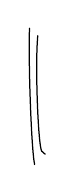
\begin{tikzpicture}[x=1cm,y=1cm,line width=.45pt,line cap=round]
\draw (0,0) .. controls (-.015,-.48) and (.025,-1.54) .. (.065,-1.73);
\draw (.105,-.095) .. controls (.070,-.48) and (.110,-1.48) .. (.155,-1.56) .. controls (.165,-1.58) and (.185,-1.59) .. (.200,-1.60);
\end{tikzpicture}}}
\margin{\unsure{recall that we assume} $\pi$ \unsure{anabelian|nonabelian}
$(2g+\nu\geq3)$}
\[
1\longrightarrow\pi'\longrightarrow
\widehat{\widehat{\mathcal T}}(\pi,i)\longrightarrow
\unsure{\widehat{\widehat{\mathcal G}}}(\pi',i)\longrightarrow1
\]
or again
\[
1\longrightarrow\widehat{\pi}_{g,\nu-1}\longrightarrow
\widehat{\widehat{\mathcal T}}_{g,(\nu,\nu-1)}
\longrightarrow\unsure{\widehat{\widehat{\mathcal G}}}_{g,\nu-1}
\longrightarrow1
\]
which contains the exact sequence
\[
1\longrightarrow\pi_{g,\nu-1}^{\unsure{*|+}}\longrightarrow
\mathcal T_{g,(\nu,\nu-1)}\longrightarrow
\unsure{\mathcal G}_{g,\nu-1}\longrightarrow1
\]
\unsure{as|known} sub\deleted{\unsure{particular|dense part}}, \unsure{sequence|is} exact.
It is convenient to work instead with
\diagram{\begin{tikzcd}[ampersand replacement=\&,column sep=2.1em,row sep=3.0em]
1 \arrow[r,dash] \&
\pi_{g,\nu-1} \arrow[r,dash] \arrow[d,hook',no head] \&
\unsure{\mathcal T}_{g,\nu}^{!+} \arrow[r] \arrow[d,hook',no head] \&
\mathcal G_{g,\nu-1}^{!+} \arrow[r,dash] \arrow[d,hook',no head] \& 1 \\
1 \arrow[r,dash] \&
\widehat{\pi}_{g,\nu-1} \arrow[r] \arrow[d,equal] \&
\underset{\deleted{\unsure{\illegible{1}}}}{\widehat{\mathcal T}_{g,\nu}^{!+}}
\arrow[r] \arrow[d,hook',no head] \&
\widehat{\mathcal G}_{g,\nu-1}^{!+} \arrow[r,dash] \arrow[d,hook'] \& 1 \\
1 \arrow[r,dash] \&
\widehat{\pi}_{g,\nu-1} \arrow[r] \&
\widehat{\widehat{\mathcal T}}_{g,\nu}^{!} \arrow[r] \&
\widehat{\widehat{\mathcal G}}_{g,\nu-1}^{!} \arrow[r,dash] \& 1
\end{tikzcd}}

The map $\unsure{\text{Prediscretifications}|\text{Prediscretifications}}^{+}(\pi)\longrightarrow
\unsure{\text{Prediscretifications}|\text{Prediscretifications}}^{+}(\pi')$ is thus identified with
$\widehat{\widehat{\mathcal T}}_{g,\nu}^{!}/\widehat{\mathcal T}_{g,\nu}^{!}$,
we read off the diagram that this is
$\simeq\widehat{\widehat{\mathcal G}}_{g,\nu-1}^{\unsure{!}\deleted{\unsure{+}}}/
\widehat{\mathcal G}_{g,\nu-1}^{!+}$,
whence bijectivity on the sets of oriented prediscretifications.

In the group $\widehat{\widehat{\mathcal T}}_{g,\nu}^{!}=\mathcal T$,
we have an invariant subgroup $\widehat{\pi}_{g,\nu-1}=\pi'$,
and a subgroup $\Sigma$ $(\unsure{=|\longleftarrow}\widehat{\mathcal T}_{g,\nu}^{!+})$
\mspage{347}

\scanpage{349}

between $\pi'$ and $\mathcal T$, \deleted{\unsure{giving by}} \inserted{giving} a subgroup $\Sigma'\simeq\mathcal T(\pi')$\inserted{$(=\unsure{\widehat{\mathcal G}^{!+}_{g,\nu-1}})$} in $\unsure{\mathcal T'}=\mathcal T/\pi'$ $(\simeq\widehat{\widehat{\mathcal G}}^{!}_{g,\nu-1})$, and we know well that then
\[
\mathcal T/\Sigma\simeq\mathcal T'/\Sigma',
\]
and \deleted{$\unsure{N(\Sigma)}$} that the normalizer \inserted{$\mathcal N$,} of $\Sigma$ in $\mathcal T$ is the inverse image of the normalizer $\mathcal N'$ of $\Sigma'$ in $\mathcal T'$, so that $\mathcal N/\Sigma\simeq\mathcal N'/\Sigma'$, which proves what we wanted.

\uline{Corollary} We have canonical \unsure{isomorphisms}
\[
\Gamma_{g,\nu}\xrightarrow{\sim}\Gamma_{g,\nu-1}\xrightarrow{\sim}\unsure{\cdots}\quad\deleted{\unsure{\Gamma_{g,0}}}
\]
\margin{We also see that $\unsure{\Sigma|\Sigma^{!}}$ invariant in $\unsure{\mathcal T|\widehat{\widehat{\mathcal T}}}$ is equivalent to $\Sigma'$ invariant in $\widehat{\widehat{\mathcal T}}'$}
so that if $g\geq2$, we have \unsure{canonically} $\Gamma_{g,\nu}\simeq\Gamma_{g,0}$, on the other hand $\Gamma_{1,\nu}\simeq\Gamma_{1,1}$ $(g=1,\nu\geq1)$, $\Gamma_{0,\nu}\simeq\Gamma_{0,3}$ $(\nu\geq3)$.

\uline{N.B.} The ``fact'' \deleted{\illegible{1}} assumed is far from obvious --- even that $\widehat{\widehat{\mathcal T}}^{\unsure{!}}_{g,(\nu,\nu-1)}\longrightarrow\unsure{\widehat{\widehat{\mathcal T}}_{g,\nu-1}|\widehat{\widehat{\mathcal M}}_{g,\nu-1}}$ is surjective, or that $\widehat{\widehat{\mathcal T}}_{g,(\nu,\nu-1)}\longrightarrow\widehat{\widehat{\mathcal G}}_{g,\nu-1}$ is injective, is far from obvious, and is perhaps altogether false !

The assumed fact amounts to a statement of the existence of a functor \unsure{in} the opposite direction ``drilling holes'', \unsure{which|what} in any case remains not understood.

\mspage{348}

\scanpage{350}
\mspage{177}

28. \uline{Change of type} $(g,\nu)$ \unsure{(continued)} : \uline{\unsure{passage} to a finite covering.}

Let $\pi$ be a profinite group \inserted{with loops} of type $(g,\nu)$, anabelian as always, $\pi'$ a subgroup of finite index. We know (\unsure{or we|we thereby} verify, by passing to the discrete case) that \deleted{\illegible{1} \unsure{discretified}} \inserted{equipped with the} \unsure{traces} \unsure{on|under} $\pi$ of the \unsure{loop} subgroups of $\pi$, $\pi'$ is a group with loops.

\deleted{If for every $i\in I(\pi)$, we consider an $L_i$, and the $\unsure{n}$ conjugates $\unsure{\operatorname{int}(g)}L_i$ \inserted{$=L_{i\alpha}$}, with $g\in\pi\bmod\pi'$ $(n=[\pi:\pi']\unsure{\}},\ \deleted{\unsure{n}}\ \inserted{1\leq\alpha\leq n})$ \deleted{\unsure{counted|to count} the number of times that a conjugacy class in $\pi'$ of the subgroup $\unsure{\operatorname{int}(g)}L_i$ is} \inserted{then if $\unsure{d_{\alpha}|d_{i\alpha}}=[L_{i\alpha}:\unsure{L'_{i\alpha}|N'_{i\alpha}}\deleted{\unsure{\cap\pi'}}]$ \unsure{for} $L'_{i\alpha}=L_{i\alpha}\cap\pi'$, then} exactly $d_{i\alpha}$ among the $L'_{i\beta}$ \inserted{$(1\leq\beta\leq n)$} are conjugate in $\pi'$ to $L'_{i\alpha}$, and if we sum over the distinct \unsure{conjugacy} classes of the subgroups}

The loop subgroups are \unsure{also|thus} the \deleted{\unsure{the}} subgroups $L'$ such that
\[
\text{a)}\quad L'=\operatorname{Centr}_{\pi}(L')\cap\pi'.
\]
\[
\text{b)}\quad L\unsure{=|:}\operatorname{Centr}_{\pi}(L')\text{ is a \unsure{loop} subgroup in }\pi.
\]
We put $d(L')=[L:L']$, and we thus have a function
\[
d:I'=I(\pi')\longrightarrow\mathbb N^*,
\]
and a map $I'\xrightarrow{\varphi}I$, such that $\forall i\in I$, we have
\[
\text{(1)}\qquad \sum_{\substack{i'\in I'\\\text{over }i}}d(i')=n
\qquad (\text{\unsure{where|here}}\ n=[\pi:\pi'])
\]
We will have the Hurwitz formula
\[
\text{(2)}\qquad \deleted{\unsure{2g|2\alpha}}\ 2g'-2=n(2g-2)+\overbrace{\sum_{i'\in I'}(d(i')-1)}^{\inserted{n\operatorname{card}I-\operatorname{card}I'}}
\]
\mspage{349}
